% Generated by jats2tex@0.11.1.0
\documentclass{article}
\usepackage{scielo}

\newcommand{\journalid}{Rev Saude Publica}
\newcommand{\journaltitle}{Revista de Saúde Pública}
\newcommand{\abbrevjournaltitle}{Rev. Saúde Pública}
\newcommand{\issnppub}{0034-8910}
\newcommand{\issnepub}{1518-8787}
\newcommand{\publishername}{Faculdade de Saúde Pública da Universidade de São
Paulo}
\newcommand\articledoi{\textsc{doi} 10.1590/S0034-8910.2014048004822}
\def\subject{Artigos Originais}
\title{Homicídios e disputas territoriais nas favelas do Rio de
Janeiro\titlegroup{}}
\author[{I}]{Barcellos, Christovam}
\author[{II}]{Zaluar, Alba}
\affil[i]{Fundação Oswaldo Cruz}
\affil[ii]{Universidade do Estado do Rio de Janeiro}
\def\authornotes{Correspondência | Correspondence: Christovam Barcellos.
\textsc{icict}/Fiocruz. Av. Brasil, 4365 Manguinhos. 21045-900 Rio de Janeiro, RJ,
Brasil. E-mail: xris@fiocruz.br
Os autores declaram não haver conflito de interesses.}
\date{ 02 2014}
\def\volume{48}
\def\issue{1}
\def\fpage{94}
\def\lpage{102}
\newcommand{\cclicense}{\ccbync}
\newcommand{\kwdgroup}{Mortalidade, Registros de Mortalidade, Coeficiente de
Mortalidade, Homicídio, estatística \&amp; dados numéricos, Violência, Áreas de
Pobreza, Territorialidade, Análise Espacial}
\newcommand{\kwdgroupes}{Mortalidad, Registros de Mortalidad, Tasa de
Mortalidad, Homicídio, estadística \&amp; datos numéricos, Violência, Áreas de
Pobreza, Territorialidad, Análisis Espacial}
%%% Nota fn1 %%%%%%%%%%%%%%%%%%%%%%%%%%%%%%%%%%%%%%%%%%%%%%%%%%%%%%%%
\expandafter\newcommand\csname fn1\endcsname{
O \textsc{ibge} classifica os setores censitários como aglomerado subnormal o conjunto de
unidades habitacionais carentes de serviços públicos essenciais, ocupando ou
tendo ocupado, até período recente, terreno de propriedade alheia (pública ou
particular) e estando dispostas, em geral, de forma desordenada e densa. Esses
critérios correspondem, na cidade do Rio de Janeiro, às favelas.}
%%% Nota fn2 %%%%%%%%%%%%%%%%%%%%%%%%%%%%%%%%%%%%%%%%%%%%%%%%%%%%%%%%
\expandafter\newcommand\csname fn2\endcsname{
As principais facções de tráfico na cidade do Rio de Janeiro são os Amigos dos
Amigos (\textsc{ada}), Comando Vermelho (CV) e Terceiro Comando Puro (\textsc{tcp}). Milícias são
organizações criminosas paramilitares que são formadas predominantemente por
policiais militares, bombeiros e agentes penitenciários que prestam serviços de
segurança privada a comerciantes locais e moradores, cobram taxas para
utilização de serviços (pedágios) ou controlam atividades econômicas ilegais,
como o jogo eletrônico e o sinal pirata da TV a cabo. Alguns territórios de
favelas permanecem fora do domínio de facções e milícias, sendo considerados
‘neutros’ aqui.}
%%% Nota fn3 %%%%%%%%%%%%%%%%%%%%%%%%%%%%%%%%%%%%%%%%%%%%%%%%%%%%%%%%
\expandafter\newcommand\csname fn3\endcsname{
Os domínios cobrem todas as favelas onde facções do tráfico ou milícias exercem
seu poder. Esses domínios podem ser exercidos com a exibição de armas ou não.
Com ou sem tráfico serve para diferenciar as favelas neutras ou dominadas por
milícias daquelas dominadas por facções do tráfico.}
%%% Nota fn4 %%%%%%%%%%%%%%%%%%%%%%%%%%%%%%%%%%%%%%%%%%%%%%%%%%%%%%%%
\expandafter\newcommand\csname fn4\endcsname{
Projetos financiados pela Fundação de Amparo à Pesquisa do Estado do Rio de
Janeiro (\textsc{faperj} – Processo E-26/110.302/2010) e Conselho Nacional de
Desenvolvimento Científico e Tecnológico (\textsc{cnp}q – Processo 482431/ 2010-5).}

\begin{document}
\selectlanguage{portuges}
\newcommand{\lingua}{Português}
\maketitle
\tableofcontents

Homicidios e disputas territoriales en las barriadas de Rio de Janeiro
\begingroup
\renewcommand{\section}[1]{\subsection*{#1}}

\begin{abstract}
\section{\textsc{objetivo}}

: Avaliar o risco de homicídios em favelas do Rio de Janeiro, considerando as
disputas territoriais em curso na cidade.

\section{\textsc{métodos}}

: O estudo baseou-se em dados de mortalidade por homicídios na cidade do Rio de
Janeiro, de 2006 a 2009. Foram avaliados os riscos em favelas e seus entornos,
em função da sua localização e do domínio por grupos armados e tráfico de
drogas. Foram empregados métodos e conceitos da geografia e etnografia, com as
abordagens de observação participante, entrevistas e análise de dados
secundários de saúde.

\section{\textsc{resultados}}

: As taxas de mortalidade por homicídios no interior das favelas foram
equivalentes ou mesmo menores que o restante da cidade, mas consideravelmente
maiores nos arredores das favelas, sobretudo em zonas de conflito entre domínios
armados rivais.

\section{\textsc{conclusões}}

: A presença do tráfico armado em zonas estratégicas da cidade aumenta as taxas
de mortalidade por violência e promove a “ecologia do perigo” no entorno de
favelas.

\ifdef{\kwdgroup}{\iflanguage{portuges}{\medskip\noindent\textbf{Palavras-chave:} \kwdgroup}{}}{}
\ifdef{\kwdgroupen}{\iflanguage{english}{\medskip\noindent\textbf{Keywords:}
\kwdgroupen}{}}{}
\ifdef{\kwdgroupes}{\iflanguage{spanish}{\medskip\noindent\textbf{Palavras
claves:} \kwdgroupes}{}}{}
\ifdef{\kwdgroupfr}{\iflanguage{french}{\medskip\noindent\textbf{Mots clés:}
\kwdgroupfr}{}}{}
\end{abstract}
\endgroup

\begingroup
\renewcommand{\section}[1]{\subsection*{#1}}
\begin{otherlanguage}{spanish}

\begin{abstract}
\section{\textsc{objetivo}}

: Evaluar el riesgo de homicidios en barriadas de Rio de Janeiro, considerando
las disputas territoriales en curso en la ciudad.

\section{\textsc{métodos}}

: El estudio se basó en datos de mortalidad por homicidios en la ciudad de Rio
de Janeiro, de 2006 a 2009. Se evaluaron los riesgos en barriadas y sus
entornos, en función de su localización y del dominio por grupos armados y
tráfico de drogas. Se emplearon métodos y conceptos de la geografía y
etnografía, con los abordajes de observación participante, entrevistas y
análisis de datos secundarios de salud.

\section{\textsc{resultados}}

: Las tasas de mortalidad por homicidios en el interior de las barriadas fueron
equivalente o inclusive menores que en el resto de la ciudad, pero
considerablemente mayores en los alrededores de las barriadas, sobretodo en
zonas de conflicto entre dominios armados rivales.

\section{\textsc{conclusiones}}

: La presencia del tráfico armado en zonas estratégicas de la ciudad aumenta las
tasas de mortalidad por violencia y promueve la “ecología del peligro” en el
entorno de las barriadas.

\ifdef{\kwdgroupes}{\medskip\noindent\textbf{Palavras claves:} \kwdgroupes}{}
\end{abstract}
\end{otherlanguage}
\endgroup
\section{\textsc{introdução}}

O aumento dos homicídios nas últimas décadas evidenciou mudanças nas relações
sociais, nos valores, na visão de mundo da sociedade, exigindo nova abordagem
que permita entender esse complexo
fenômeno.\textsuperscript{[}\textsuperscript{13}\textsuperscript{]}\textsuperscript{,}\textsuperscript{[}\textsuperscript{24}\textsuperscript{]}

As violências são diferenciadas e têm múltiplas determinações, que devem ser
abordadas em diversas escalas de análise, desde o nível internacional até o
local, i.e., o da vida cotidiana.\textsuperscript{[}\textsuperscript{16}\textsuperscript{]}
Cada uma das escalas apresenta preditivos macrossociais e coletivos, bem como
componentes microssociais e subjetivos. Os primeiros são fundamentais para
identificar grupos e áreas de risco; os segundos, para a compreensão dos
processos sociais geradores da violência na sociedade pós-industrial. A
caracterização da violência apenas em termos macrossociais ou exclusivamente
subjetiva impede a compreensão do fenômeno multifacetado.

Estudos quantitativos sobre os determinantes das mortes por agressão têm se
baseado em variáveis individuais agregadas ou em variáveis ecológicas. As
variáveis agregadas recuperam o perfil socioeconômico das vítimas, como
desigualdade econômica, renda, escolaridade, estrutura familiar e gravidez na
adolescência,\textsuperscript{[}\textsuperscript{19}\textsuperscript{]}
enquanto as variáveis ecológicas correlacionam características das vizinhanças
onde viviam as vítimas, como estrutura populacional, densidade demográfica,
mobilidade habitacional, homogeneidade étnica, proporção de pobres e taxa de
desemprego.\textsuperscript{[}\textsuperscript{10}\textsuperscript{]}
A hipótese subjacente a estes estudos é que as vítimas morariam em bairros
superpovoados, etnicamente heterogêneos, com altas taxas de desemprego, com
famílias chefiadas por mulheres, gravidez na adolescência e pessoas de renda e
escolaridade baixas. Portanto, além de variáveis socioeconômicas agregadas,
fatores relacionados ao espaço urbano tornaram-se parte da investigação
criminológica.

Entre os fatores ecológicos preditivos da violência encontram-se as disputas
territoriais nas favelas, com início na década de 1980 no Rio de Janeiro, quando
apareceram divisões entre grupos armados lutando por posições na venda de drogas
ilícitas. Tais conflitos reforçaram o \textit{ethos}
de masculinidade violenta que cria disposições subjetivas para a resolução
litigiosa de conflitos.\textsuperscript{[}\textsuperscript{23}\textsuperscript{]}
As favelas passaram a ser refúgio de grupos criminosos e bolsões onde práticas
de segurança interna e de justiça informal foram moldadas de acordo com o
domínio local.

Recentemente, o desenvolvimento de tecnologias de mapeamento digital, e
particularmente dos ambientes genericamente denominados Sistemas de Informações
Geográficas (\textsc{sig}), abriu novos caminhos para investigações epidemiológicas que
têm utilizado tais técnicas para mapear e analisar a distribuição de agravos à
saúde relacionados à violência.\textsuperscript{[}\textsuperscript{2}\textsuperscript{]}\textsuperscript{,}\textsuperscript{[}\textsuperscript{6}\textsuperscript{]}\textsuperscript{,}\textsuperscript{[}\textsuperscript{18}\textsuperscript{]}
A maior parte desses métodos tem sido utilizada para avaliar a distribuição
espacial da ocorrência de agravos, identificando preditivos a partir dos padrões
espaciais. Neste estudo, ao contrário, parte-se de hipóteses prévias sobre a
distribuição dos agravos baseada na estrutura espacial, favelas e principais
vias de circulação da cidade, para avaliar o efeito desses ambientes na
distribuição da violência. Segundo Milton
Santos,\textsuperscript{[}\textsuperscript{17}\textsuperscript{]}
o espaço é constituído por um conjunto indissociável de objetos e ações. Os
objetos são fixos no espaço e determinam as ações que acontecem nele. A presença
de favelas, portanto, condicionaria as práticas sociais no seu entorno.

Poucos estudos sobre violência no Brasil foram realizados na escala local por
meio de dados desagregados, pois têm caráter macrossocial, buscando a associação
entre indicadores socioeconômicos construídos para grandes áreas como regiões
administrativas e áreas de planejamento. Vários mostraram maior risco de morte
por violência em áreas pobres das cidades, tanto em
periferias\textsuperscript{[}\textsuperscript{10}\textsuperscript{]}\textsuperscript{,}\textsuperscript{[}\textsuperscript{12}\textsuperscript{]}
como em regiões de concentração de
favelas.\textsuperscript{[}\textsuperscript{2}\textsuperscript{]}\textsuperscript{,}\textsuperscript{[}\textsuperscript{6}\textsuperscript{]}\textsuperscript{,}\textsuperscript{[}\textsuperscript{20}\textsuperscript{]}
Neste artigo procurou-se distinguir as favelas não por indicadores de pobreza,
mas segundo variáveis indicadoras da atuação de grupos armados em sangrentas
disputas.

Como vários preditivos da violência são dificilmente mensuráveis, a pesquisa
etnográfica é imprescindível. O método dos casos desdobrados permite conectar o
local às demais esferas da vida social, além de impor uma abordagem
histórica\textsuperscript{[}\textsuperscript{3}\textsuperscript{]}
que permite relacionar a mortalidade por homicídios às práticas violentas de
traficantes, policiais e milicianos em algumas favelas.

O objetivo desse estudo foi avaliar o risco de homicídios nas favelas do Rio de
Janeiro, considerando as disputas territoriais em curso na cidade.

\section{\textsc{métodos}}

As favelas foram classificadas segundo o domínio de grupos armados – milícias ou
traficantes de drogas – procurando responder às perguntas: “Existe risco maior
em viver em favelas e seus entornos?”, “Este risco depende da localização e do
domínio das favelas?”, “As disputas entre grupos armados podem aumentar este
risco?”

Os dados sobre mortalidade por homicídios de 2006 a 2009 foram obtidos por duas
fontes de informação: Sistema de Informações de Mortalidade (\textsc{sim}), da Secretaria
Municipal de Saúde do Rio de Janeiro, pela seleção dos óbitos resultantes de
intervenções legais e operações de guerra; óbitos por homicídios (\textsc{cid}10: X85 a
Y09); bem como as lesões por arma de fogo e perfuro-cortante com
intencionalidade ignorada (\textsc{cid}10: Y22 a Y24 e Y28). Este último grupo foi
incluído com o objetivo de superar as deficiências da classificação de causa do
óbito.\textsuperscript{[}\textsuperscript{5}\textsuperscript{]}
Os registros de óbitos do \textsc{sim} foram georreferenciados segundo o endereço de
residência da vítima. Os endereços foram comparados com a malha digital de
logradouros e outras bases de dados. Os endereços restantes foram
georreferenciados manualmente, contando com a experiência da equipe de campo
sobre endereços informais de favelas. Este processo permitiu a localização de
96,0\% dos registros.

A segunda fonte de informação foi o Instituto de Segurança Pública (\textsc{isp}) da
Secretaria Estadual de Segurança Pública. Foram selecionados os registros de
agressões ocorridos envolvendo moradores do município do Rio de Janeiro, entre
2006 e 2009 e que resultaram em morte da vítima. Neste caso, os óbitos foram
georreferenciados, usando como endereço o local de ocorrência, seja a morte,
seja o encontro do corpo.

A primeira estratégia de georreferenciamento, empregada para dados do \textsc{sim},
permitiu o cálculo de taxas de homicídio, pela razão entre o número de
homicídios por local de residência e a população total residente em cada área.
Já a segunda estratégia, usada para dados do \textsc{isp}, permitiu identificar áreas com
maior concentração de eventos violentos e fatais que,segundo as hipóteses deste
trabalho, estariam relacionadas aos conflitos armados na cidade.

Para a estimativa da população residente foram utilizados os dados do censo
demográfico de 2010, tendo como unidade mínima de agregação o setor censitário.
As favelas são assim classificadas segundo dois órgãos que utilizam critérios
diferentes: pelo Instituto Pereira Passos (\textsc{ipp}) da Prefeitura do Rio de Janeiro,
que mantém um cadastro sobre áreas de carência social, e o Instituto Brasileiro
de Geografia e Estatística (\textsc{ibge}) que as classifica como setores censitários do
tipo subnormal.\footnote{\fn1}
Partiu-se da lista de 965 favelas fornecida pelo \textsc{ipp}, compatibilizada com os
mapas de favelas gerados pela seleção de setores censitários do tipo subnormal
segundo o censo demográfico de 2010. Esta lista, com localização e nome de
favelas, foi verificada em campo, por equipe do projeto. Esta equipe também
levantou as facções de traficantes\footnote{\fn2}
ou milícias que dominavam as favelas entre janeiro de 2005 e dezembro de 2010
por meio de visitas locais e pesquisa na
internet.\textsuperscript{[}\textsuperscript{25}\textsuperscript{]}\textsuperscript{,}\textsuperscript{[}\textsuperscript{26}\textsuperscript{]}

O \textsc{sig} foi constituído com este conjunto de dados, permitindo a organização e o
tratamento de informações espaciais por meio de procedimentos computacionais.
Neste artigo, as unidades espaciais não constituem um dado \textit{a priori}, mas foram desenhadas em função das hipóteses do estudo, não coincidente com
áreas político-administrativas, mas considerando que a área de influência de um
domínio se estende a certa distância em torno das favelas dominadas pela facção
criminosa. A partir do desenho destas novas áreas, calculou-se o número de
eventos (óbitos por homicídio) dentro delas e a população total de residentes
nelas. Foi calculada a taxa de mortalidade por homicídios no entorno de favelas,
estabelecendo-se áreas de influência (\textit{buffers}
) com distâncias radiais a partir dos limites das favelas, de zero metro
(interior das favelas), de zero a 100 m, de 100 m a 250 m, de 250 m a 500 m e de
500 m a 1.000 m (entorno das favelas).

Foram incorporados dados etnográficos de pesquisas realizadas em
favelas\textsuperscript{[}\textsuperscript{21}\textsuperscript{]}
que visaram fornecer indícios que permitem inferências, pela sinergia entre
fatos sociais interconectados. Procurou-se identificar os múltiplos significados
que atores sociais emprestam às suas ações, aos riscos que correm e às relações
que estabelecem entre si nas diferentes situações de violência. Na perspectiva
de uma \textit{démarche}
reflexiva ou de um diálogo entre o cientista social e as pessoas que ele estuda,
procurou-se entender a dinâmica das situações sociais com o maior número
possível de atores.

\section{\textsc{resultados}}

A Figura~\ref{fig:f01}
mostra a população total das favelas segundo o domínio de grupos criminosos,
milícias, neutras ou sob a atuação de Unidades de Polícia Pacificadora (\textsc{upp}) ao
longo dos últimos anos, de modo a compor o quadro do resultado de vários
conflitos armados registrados na cidade em torno do domínio territorial de
favelas.

\begin{figure}
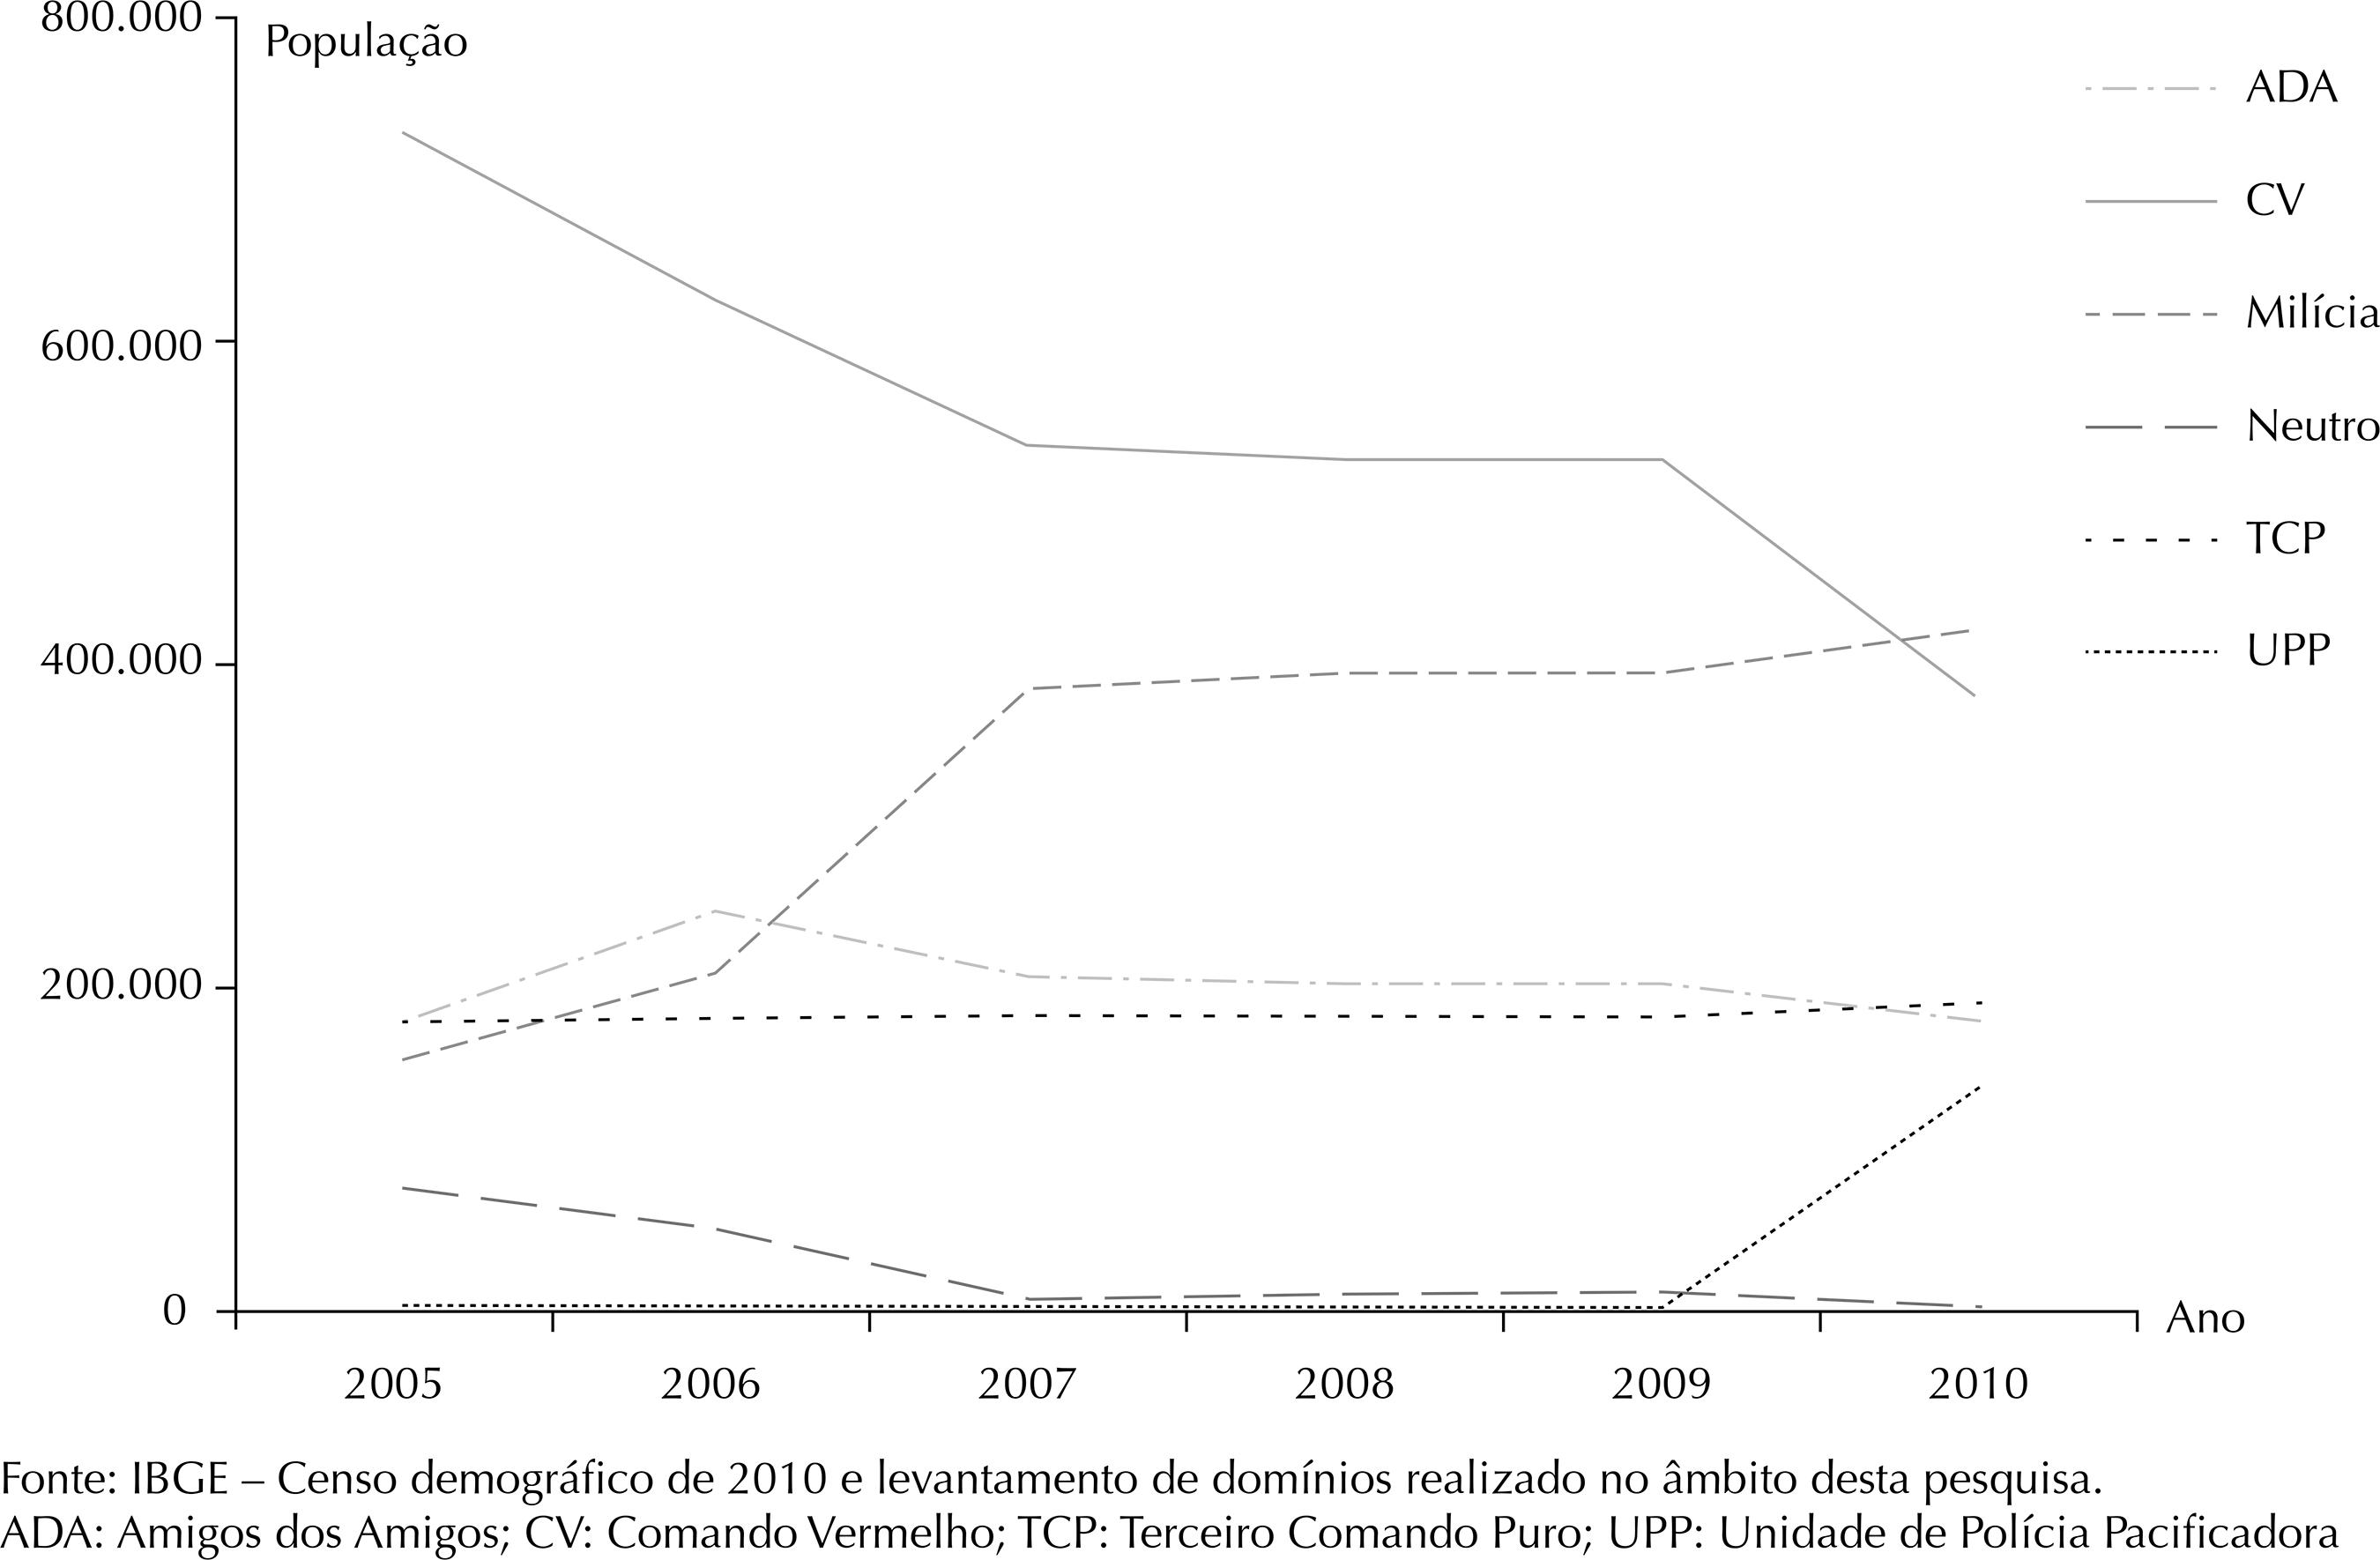
\includegraphics[width=\textwidth]{0034-8910-rsp-48-01-0094-gf01}
\caption{}\label{fig:f01}
\end{figure}

No ano de 2005 havia um claro predomínio da facção Comando Vermelho (CV) sobre
as favelas da cidade do Rio de Janeiro, abrangendo cerca de 730.000 habitantes,
quase a metade dos moradores de favelas da cidade (cerca de 1.300.000). A partir
desse ano, observa-se um decréscimo gradativo deste domínio com o avanço das
milícias e, mais recentemente, com a instalação de \textsc{upp}. Ambas as iniciativas
reduziram consideravelmente o domínio do CV, mas levaram a pequena alteração na
territorialidade de outros grupos criminosos como a facção Amigos dos Amigos
(\textsc{ada}) e Terceiro Comando Puro (\textsc{tcp}). A partir de 2005, houve também diminuição
do número de pessoas residentes em áreas neutras, grande parte agora sob o
domínio de milícias, o tipo de organização que mais ganhou territórios na
cidade.

Segundo dados de 2010, as milícias atuavam em favelas com 422.000 habitantes, o
CV dominava áreas com 377.000 habitantes, \textsc{ada} e \textsc{tcp} atuavam em áreas com 180.000
habitantes. As \textsc{upp}, instaladas nas maiores favelas a partir de 2008 e com
expansão contínua nos anos mais recentes, cobriam áreas com 142.000 habitantes,
embora estivessem presentes apenas em 7,0\% das favelas. Hoje quase inexistem
áreas neutras, livres de domínios criminosos.

A expansão das milícias se detém em algumas áreas mais próximas à Avenida
Brasil, ao aeroporto internacional e ao Porto do Rio de Janeiro, por onde chegam
armas e drogas. Estas áreas permaneceram sob o controle militar de traficantes
até recentemente, com poucas exceções, por exemplo, na Ilha do Governador, onde
está o aeroporto internacional, e áreas industriais de depósito de cargas para
empresas comerciais, junto à Avenida Brasil, que são disputadas por grupos
armados, inclusive milícias. Por causa dessas importantes atividades econômicas,
a repressão sobre os criminosos foi maior nessas áreas. Recentemente, a ocupação
de favelas nestas áreas por \textsc{upp} começou a mudar o cenário, por oferecer
segurança alternativa às das milícias.

No ano de 2009, segundo dados do \textsc{sim}, 456 pessoas residentes em favelas foram
assassinadas. Considerando que a soma de toda a população residente em favelas
no Rio de Janeiro era de cerca de 1.300.000, a taxa média de homicídios nas
favelas seria próxima de 34 por 100.000 habitantes. Este valor é menor que o
verificado para o município como um todo, com 6.320.000 habitantes e 3.260
óbitos por homicídio para o ano de 2009, o que produz um valor aproximado de 52
homicídios por 100.000. Portanto, haveria risco maior de morrer por homicídio
fora do que dentro das favelas, o que confirmaria a hipótese de que a presença
de traficantes dá segurança aos moradores delas.

Para examinar esta hipótese, taxas de mortalidade por homicídios, segundo dados
do \textsc{sim}, foram calculadas para áreas de influência em torno de favelas,
classificadas segundo o domínio. A Figura~\ref{fig:f02}
mostra as taxas de homicídios por domínio, segundo tais distâncias, no ano de
2009.

\begin{figure}
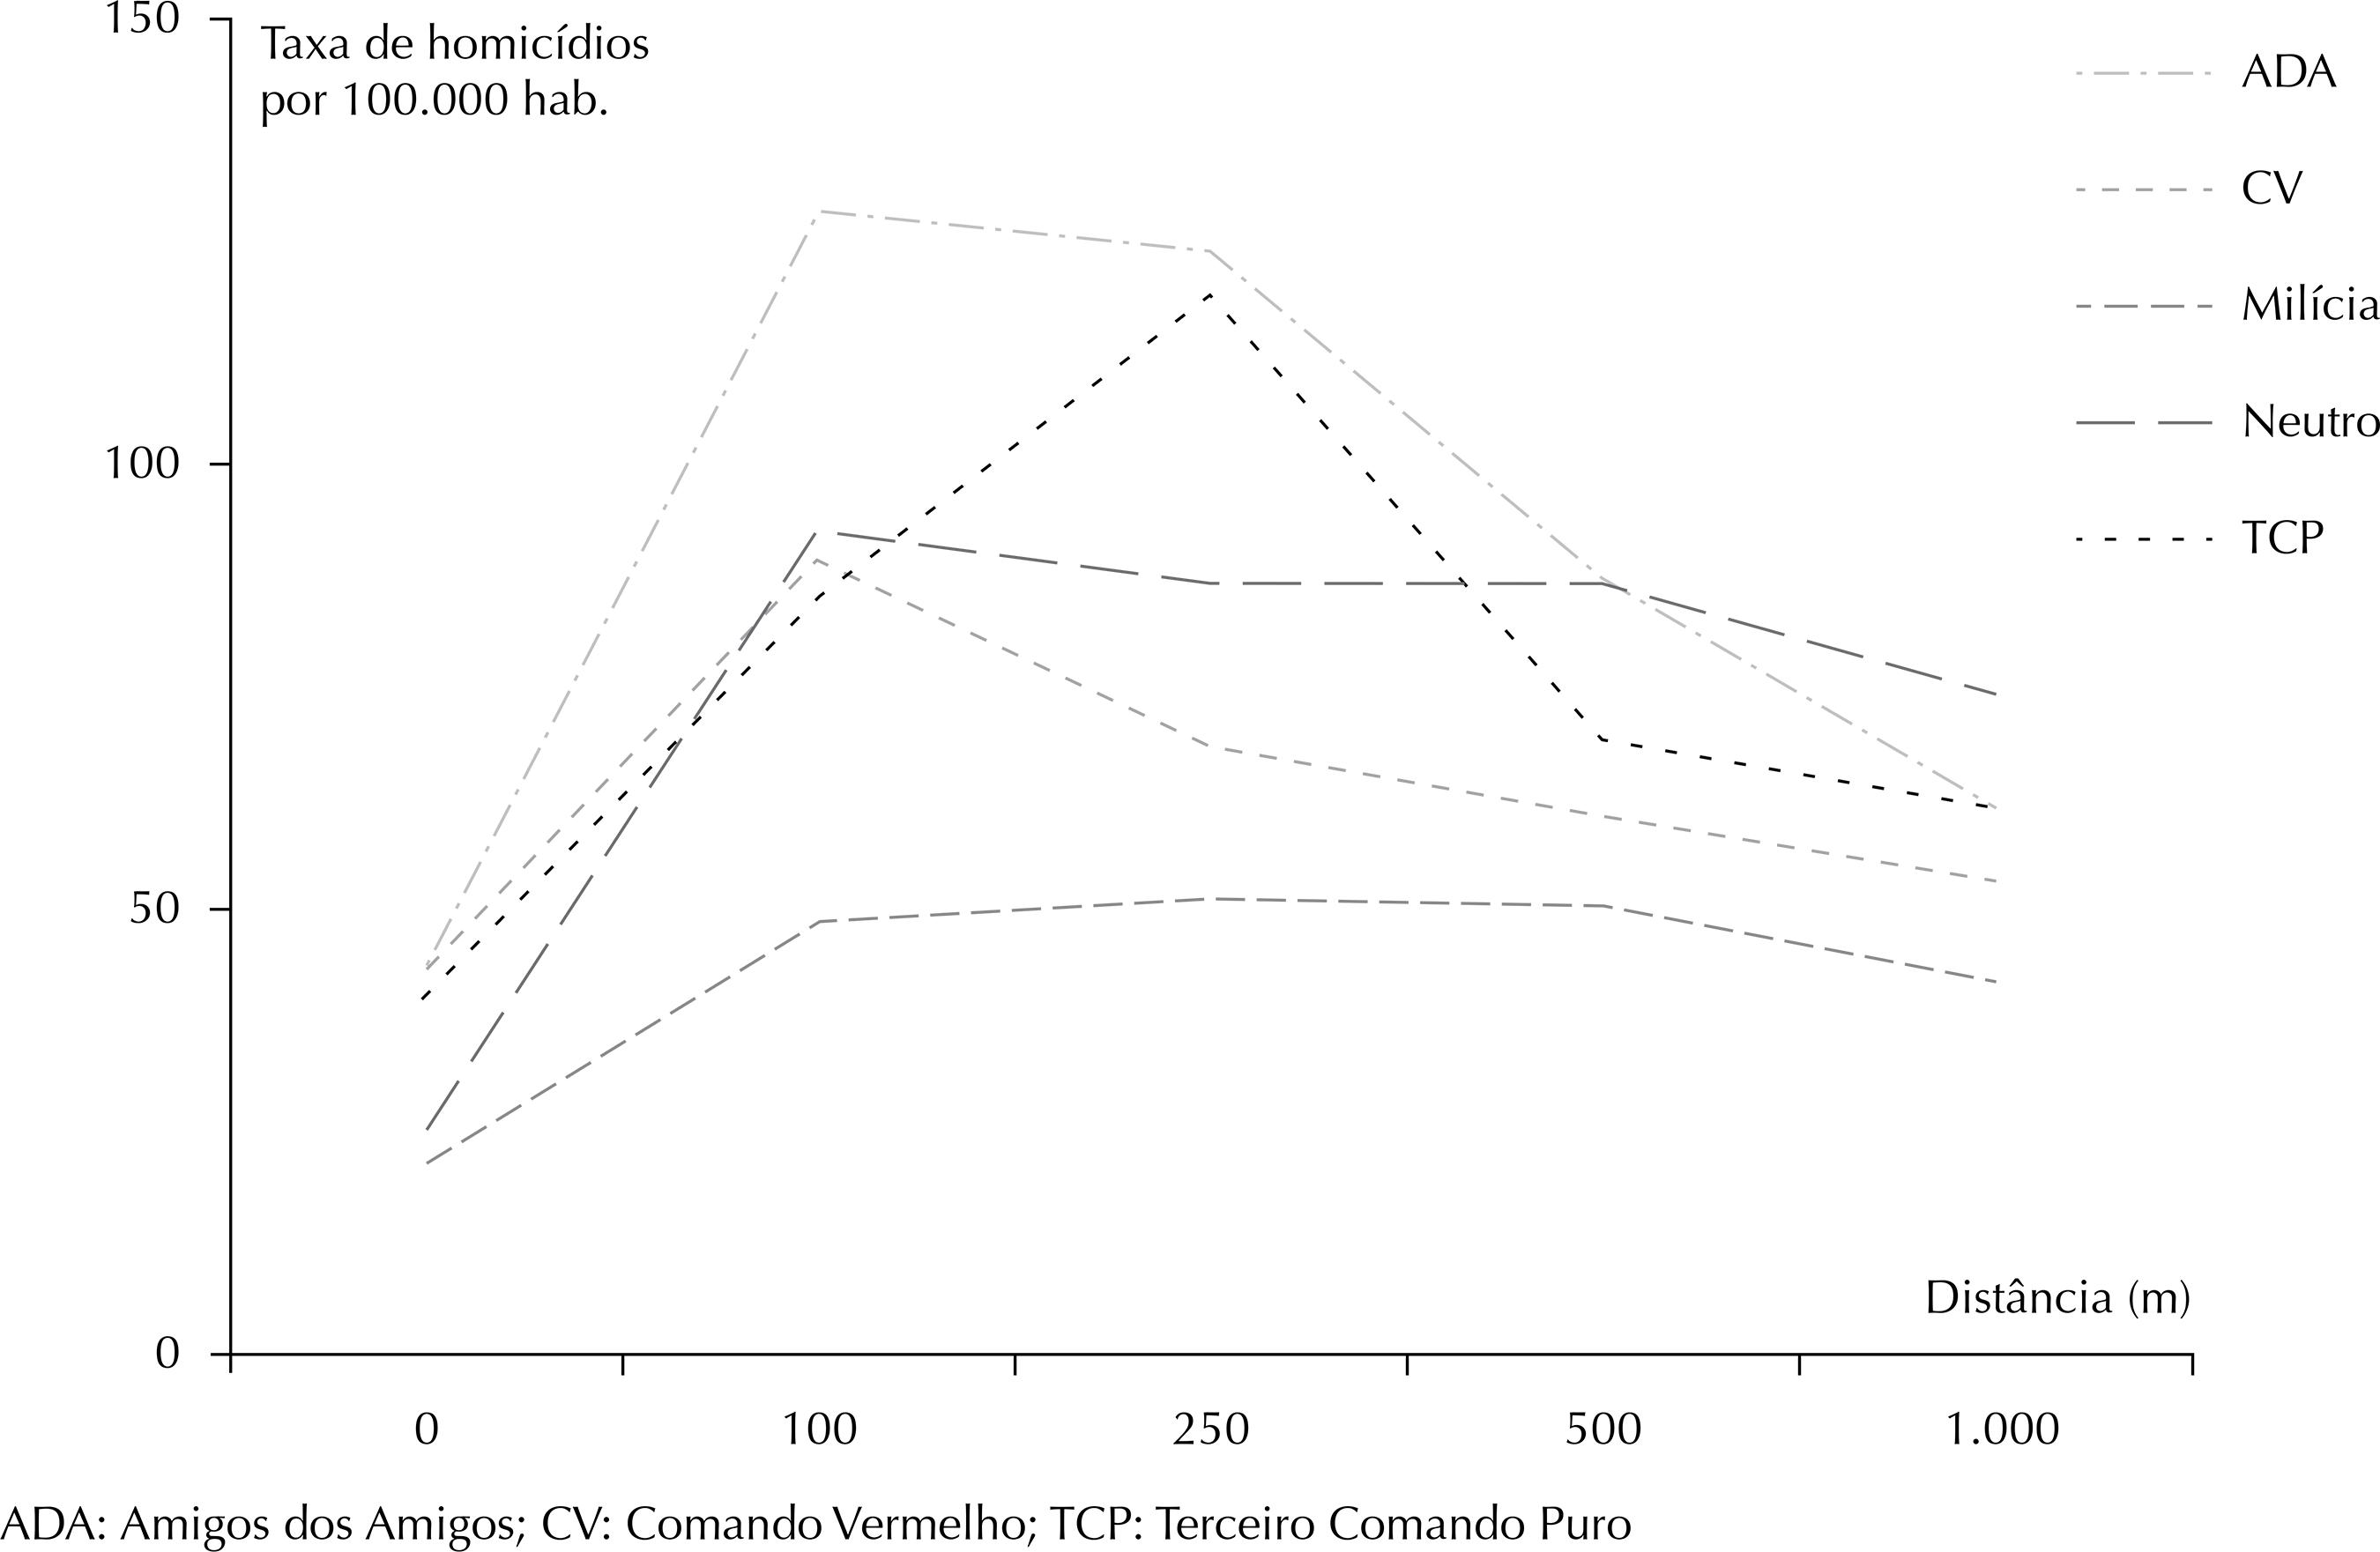
\includegraphics[width=\textwidth]{0034-8910-rsp-48-01-0094-gf02}
\caption{}\label{fig:f02}
\end{figure}

Dentro das favelas, observa-se variação de 22 a 44 homicídios por 100.000
habitantes. Ao redor das favelas, até 100 m de distância, as taxas sobem
consideravelmente, variando de 48 a 129/100.000. Para distâncias entre 100 m e
250 m, estes valores tendem a diminuir, com exceção das favelas dominadas pela
facção CV que atinge seu ápice aos 250 m e o \textsc{tcp}, que chega ao valor máximo de
119/100.000 na distância de 250 m a 500 m. As taxas de homicídio em torno de
favelas dominadas por milícias apresentam pequena variação da taxa de homicídio
em relação à distância, com valores de 22 a 48/100.000 habitantes.

Segundo estas estimativas, seria mais perigoso morar em torno de áreas ocupadas
pelos grupos \textsc{ada}, \textsc{tcp} e CV, do que nas demais áreas afastadas de favelas
dominadas por facções de traficantes ou no interior destas. Como as taxas são
sempre mais altas nos arredores de favelas que no resto da cidade, elas se
tornariam parte da “ecologia do perigo”.\textsuperscript{[}\textsuperscript{9}\textsuperscript{]}
Os estudos etnográficos mostram que nas áreas sob tais domínios, os jovens
vulneráveis são socializados pelo manejo das armas de fogo, elementos-chave da
nova “cultura de rua”, criando as áreas quentes da morte
prematura.\textsuperscript{[}\textsuperscript{11}\textsuperscript{]}
Traficantes armados, com seus impressionantes estoques de armas e munições,
apontam para o paradoxo do monopólio legítimo da violência no Brasil e a
logística inquebrantável que aporta armas e munições continuamente às quadrilhas
atuantes no varejo das favelas. Além de treiná-los para o combate, policiais e
militares corruptos, auxiliados por contrabandistas, levam armas exclusivas das
Forças Armadas brasileiras às quadrilhas de traficantes, alimentando o estado de
guerra pelo controle de pontos de venda e de territórios. Estas mesmas armas vão
matar policiais que fazem a repressão às atividades ilegais das
quadrilhas.\textsuperscript{[}\textsuperscript{4}\textsuperscript{]}\textsuperscript{,}\textsuperscript{[}\textsuperscript{24}\textsuperscript{]}

A proximidade dos domínios das milícias, ao contrário, não representaria um
sobre-risco de homicídios para os moradores. Existem diversas explicações para a
aparente proteção dos moradores de áreas dominadas pelas milícias. A ocupação
das favelas por milícias tem sido antecedida por ações de expulsão ou eliminação
de membros de facções criminosas, ou seja, a fase de maior mortalidade é
anterior ao seu domínio territorial. As milícias forçam o desarmamento, gerando
a redução de casos de violência armada, mesmo por motivações pessoais como briga
entre vizinhos e casais.\textsuperscript{[}\textsuperscript{4}\textsuperscript{]}\textsuperscript{,}\textsuperscript{[}\textsuperscript{25}\textsuperscript{]}
Além disso, as favelas dominadas por milícias na Zona Oeste, não têm limites tão
abruptos quanto na Zona Sul, resultante do processo de segregação espacial. As
atividades das milícias se estenderiam além das favelas, ocupando pontos
comerciais legais ou ilegais, como o controle de venda de gás em botijão,
transportes alternativos e jogos
eletrônicos.\textsuperscript{[}\textsuperscript{25}\textsuperscript{]}

Nas áreas dominadas pelo tráfico, é mais frequente ouvir tiros, agressão entre
pessoas, indivíduos sendo mortos ou levados à força, pessoas traficando ou
usando drogas. Nessas favelas, o número de entrevistados que afirmou ter visto
venda de drogas em sua vizinhança foi mais que o triplo (45,0\%) dos
entrevistados de favelas dominadas por milícias (14,9\%). Este resultado mostra
que a tolerância dos moradores, forçada ou não, e a convivência com o uso e
tráfico de drogas são várias vezes maiores nessas favelas. Isso indica que um
dos objetivos claros das milícias é coibir o uso e tráfico de drogas, mas sem
eliminá-lo, e proibir as armas.

As favelas foram classificadas segundo o tipo de ocupação, verificando o domínio
de grupos armados,\footnote{\fn3}
inclusive as facções do tráfico. Os resultados são apresentados na Tabela.

No raio até 250 m de favelas com presença de grupos armados, os valores
estimados para as taxas de homicídio, segundo dados do \textsc{sim}, são ligeiramente
maiores que em áreas desarmadas (45/100.000 habitantes). As maiores diferenças
surgem da comparação entre áreas com tráfico, que apresentam taxas até três
vezes superiores a favelas sem tráfico. Também as áreas onde o CV foi
recentemente desarticulado, principalmente no Complexo do Alemão, a taxa de
26,8/100.000 habitantes é consideravelmente inferior à média do município
(52/100.000 habitantes).

O \textsc{sig} foi usado para calcular distâncias entre favelas próximas ao local de
ocorrência da agressão que gerou o homicídio, segundo dados do \textsc{isp}. De um total
de 3.260 homicídios entre residentes no município, 1.093 ocorreram nas áreas
próximas a pelo menos duas favelas. As áreas situadas entre favelas de domínio
comum, i.e., ambas do CV, apresentaram a maior frequência de ocorrência de
homicídios: 386. Já as áreas de conflito potencial entre domínios, i.e.,
cercadas por duas favelas com domínios diferentes, apresentaram 355 homicídios,
o que não é pouco, pois estas áreas de interface são raras e pequenas. Esses
homicídios são mais frequentes em áreas onde se aproximam os domínios do CV e
milícia. Onde só há milícias, registrou-se 219 homicídios.

Um dos exemplos desses conflitos verifica-se na Zona Oeste, no bairro de Fazenda
Botafogo. A Figura~\ref{fig:f03}
mostra a ocorrência de homicídios nesta área, onde grupos como o CV, \textsc{ada} e
milícias dominam favelas muito próximas entre si. Nesta região também se
encontram grandes depósitos de empresas de eletrodomésticos, sempre alvos de
assaltos aos seus caminhões.\textsuperscript{[}\textsuperscript{23}\textsuperscript{]}
Por isso, também ali se instalaram milícias, o que tornou a área ainda mais
conflituosa.\textsuperscript{[}\textsuperscript{25}\textsuperscript{]}

\begin{figure}
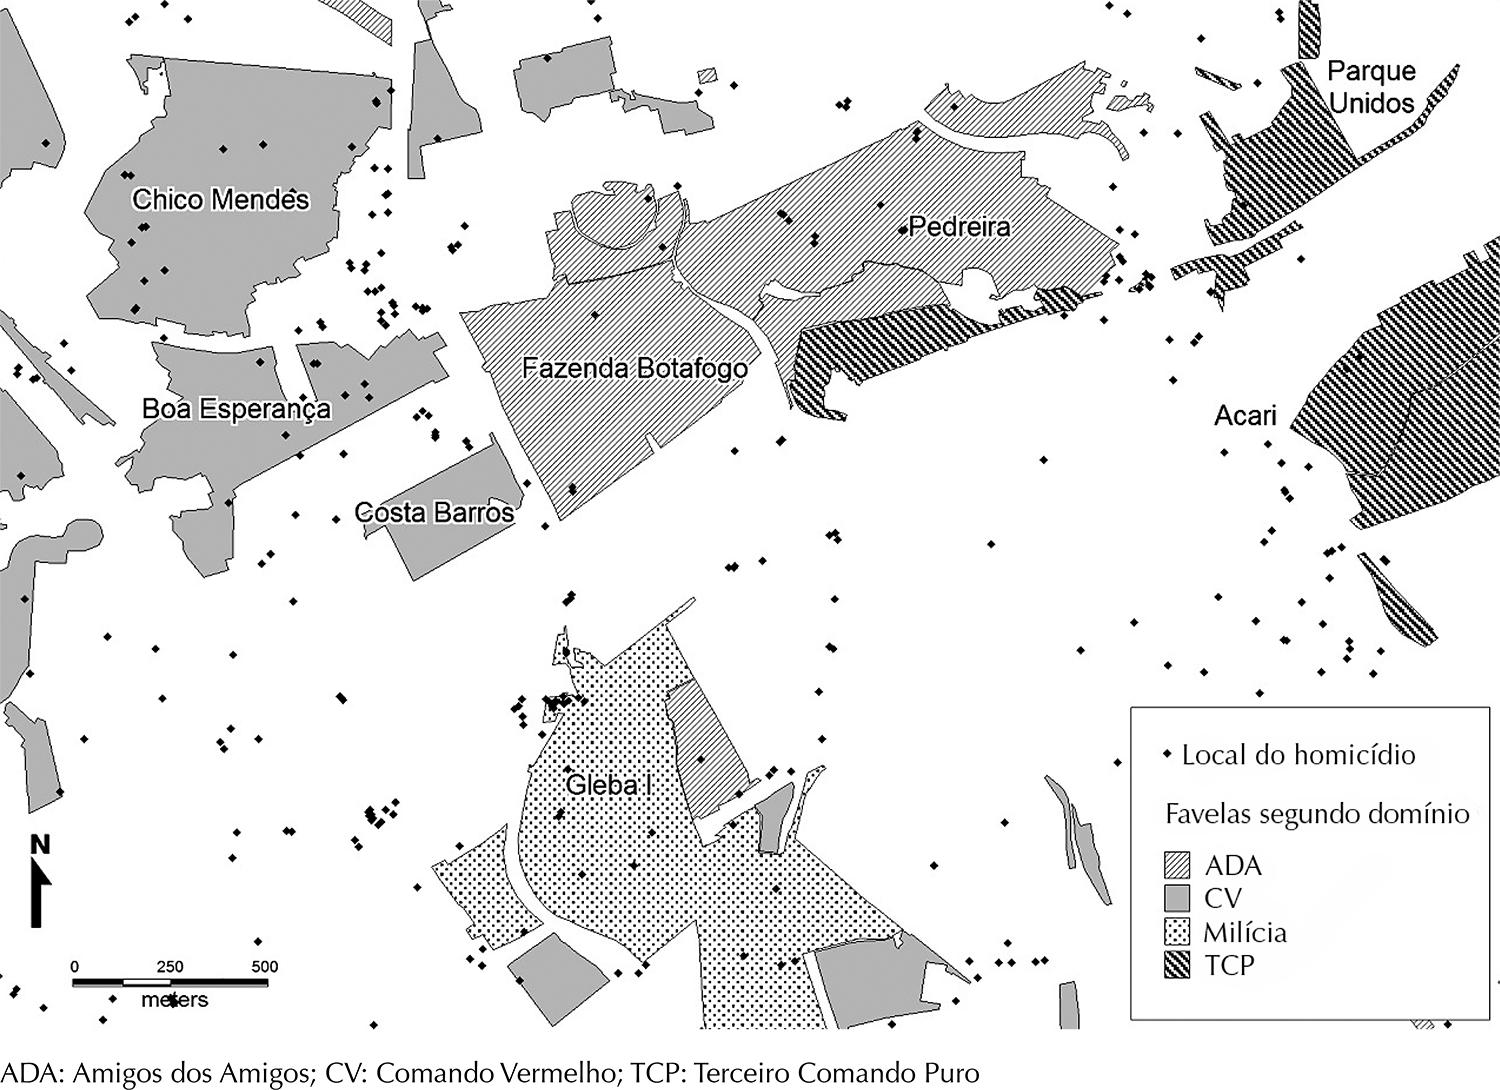
\includegraphics[width=\textwidth]{0034-8910-rsp-48-01-0094-gf03}
\caption{}\label{fig:f03}
\end{figure}

No interior das favelas observa-se ocorrência de violências resultantes em
homicídios, segundo dados do \textsc{isp}. No entanto, estes se concentram principalmente
em torno de corredores de circulação do bairro. Estes corredores constituem
zonas de contato entre os diferentes grupos, onde são frequentes os conflitos
armados, bem como a “desova” de corpos de pessoas executadas por eles.

Tais dados indicam a importância da luta por territórios dos diferentes grupos
na promoção da violência. Por outro lado, grandes áreas dominadas pelos mesmos
grupos armados, não garantem a ausência ou redução de homicídios. Estes
corredores, mesmo entre favelas sob o mesmo domínio são áreas de possíveis lutas
entre subgrupos e de violências contra comerciantes e moradores como estratégia
de manutenção de poder sobre o território.

\begin{figure}
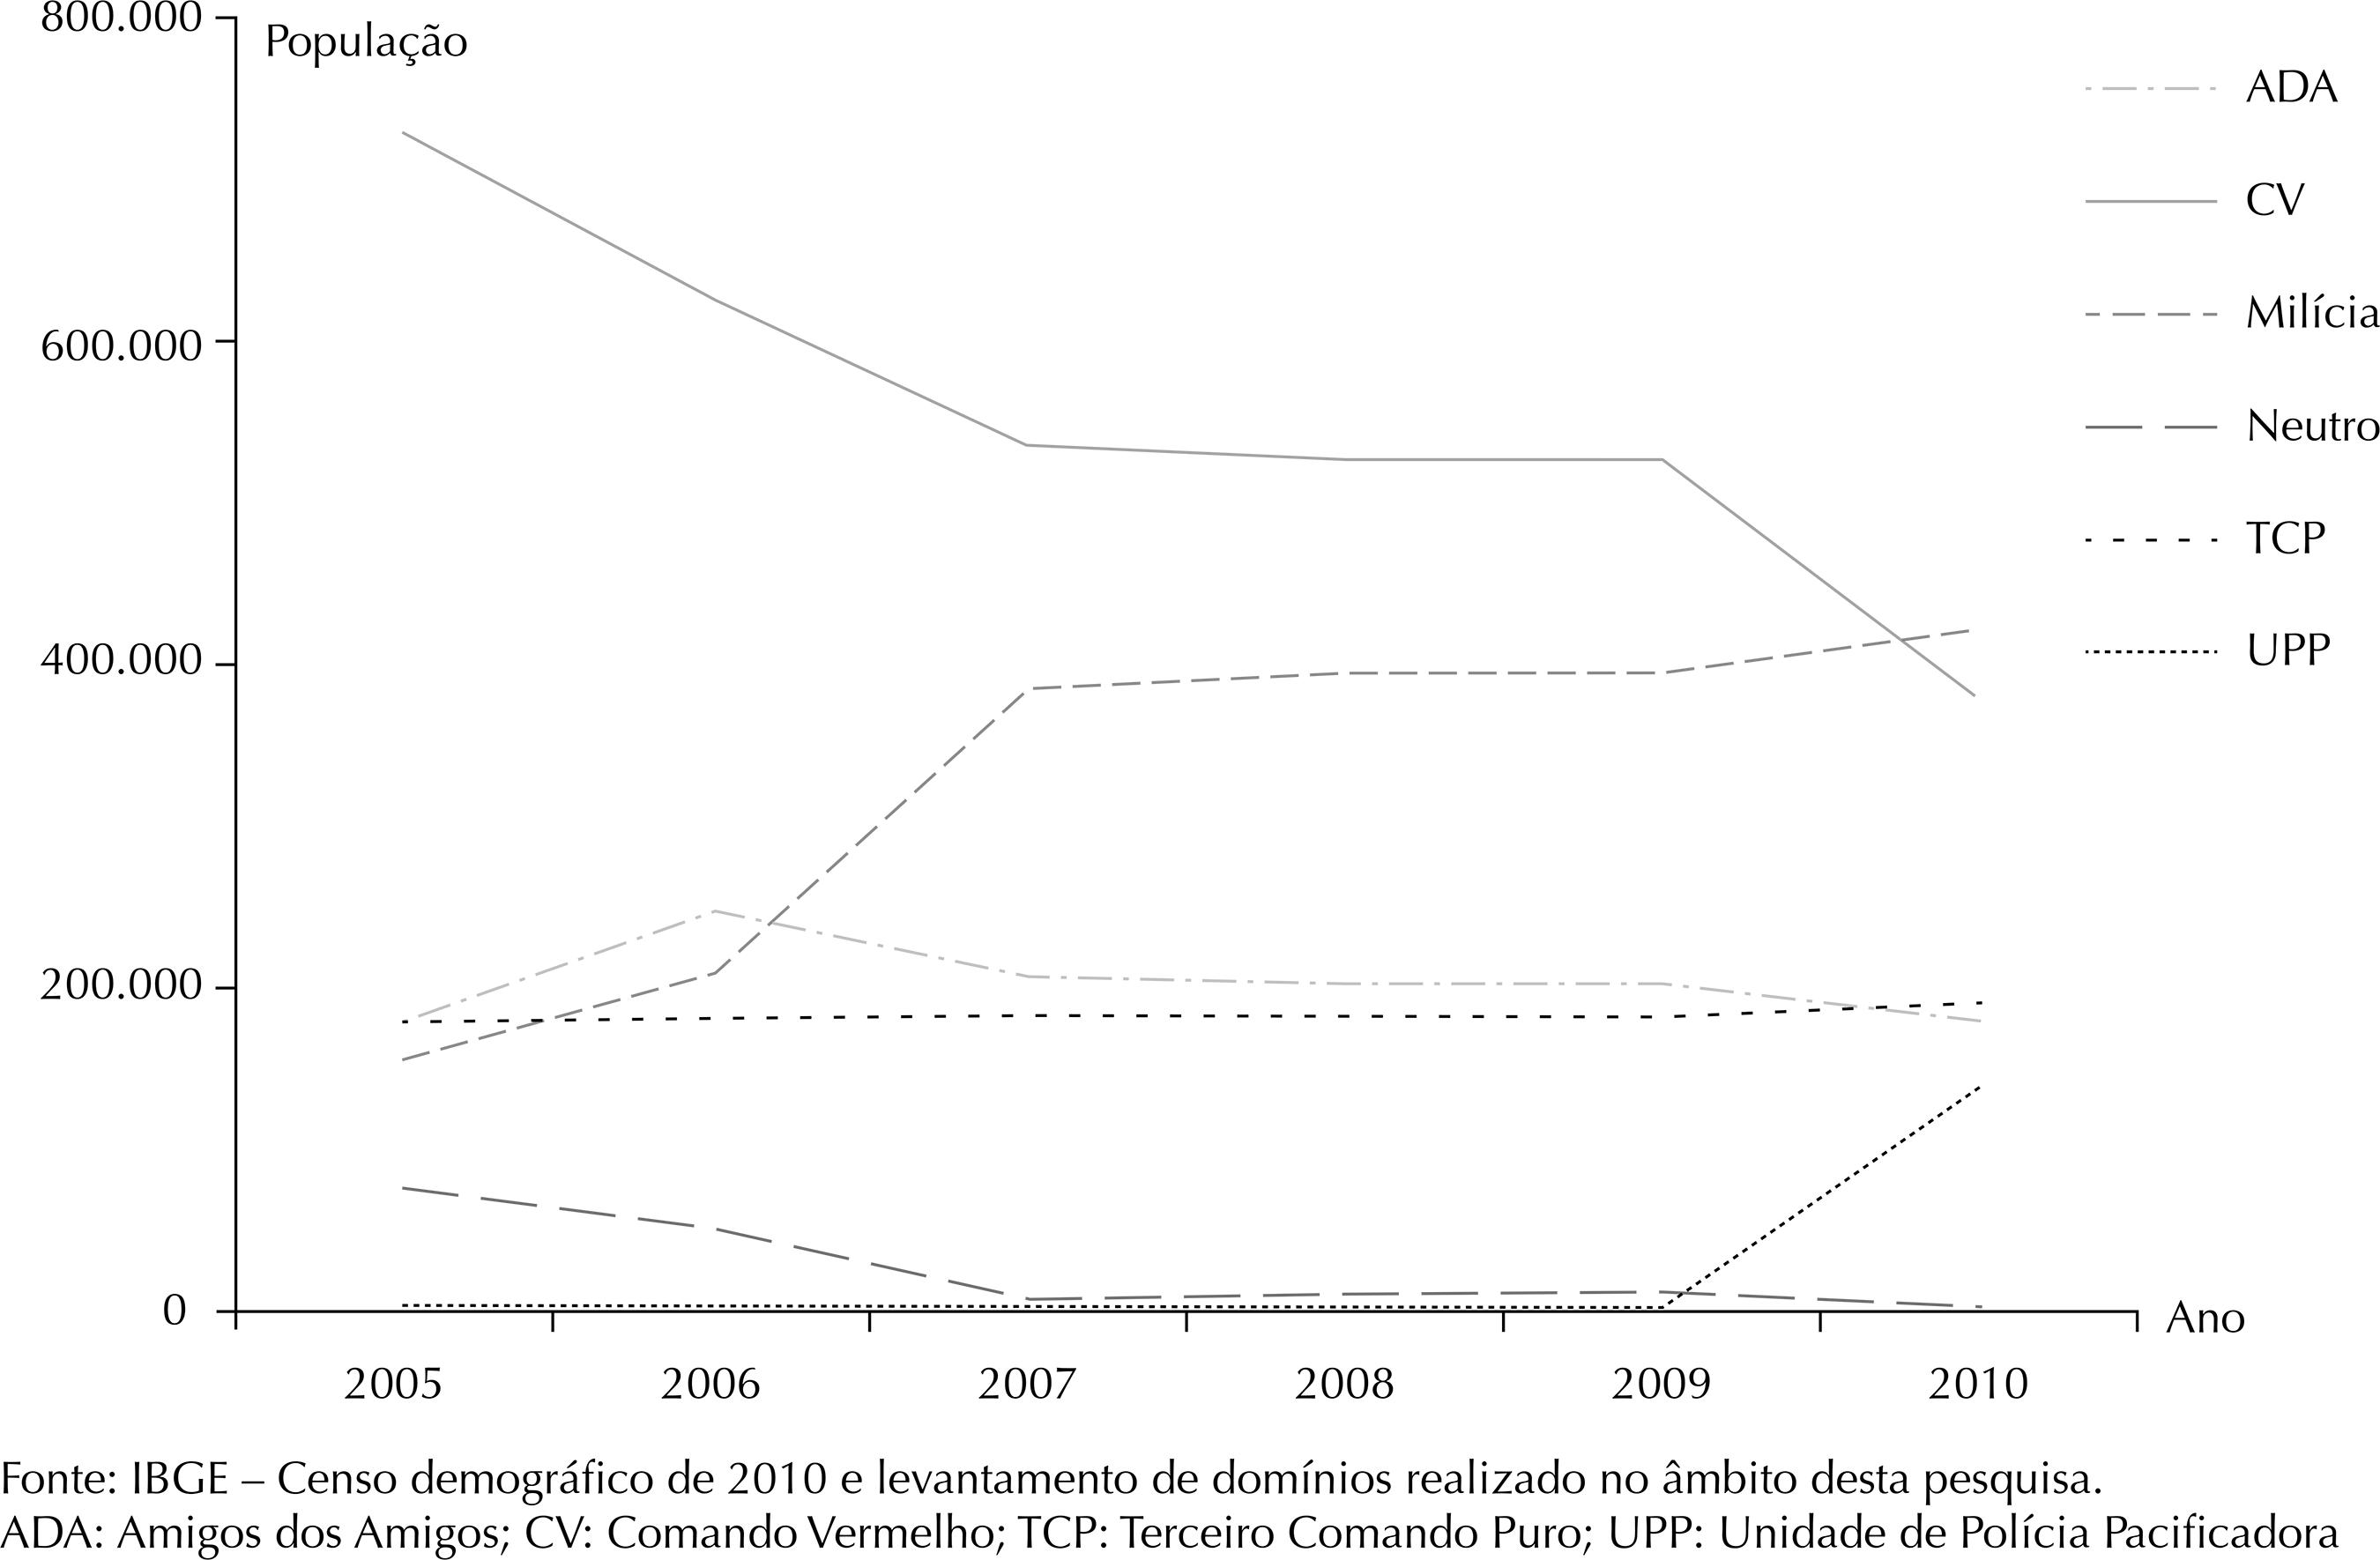
\includegraphics[width=\textwidth]{0034-8910-rsp-48-01-0094-gf01}
\caption{}\label{fig:f01}
\end{figure}
\begin{figure}
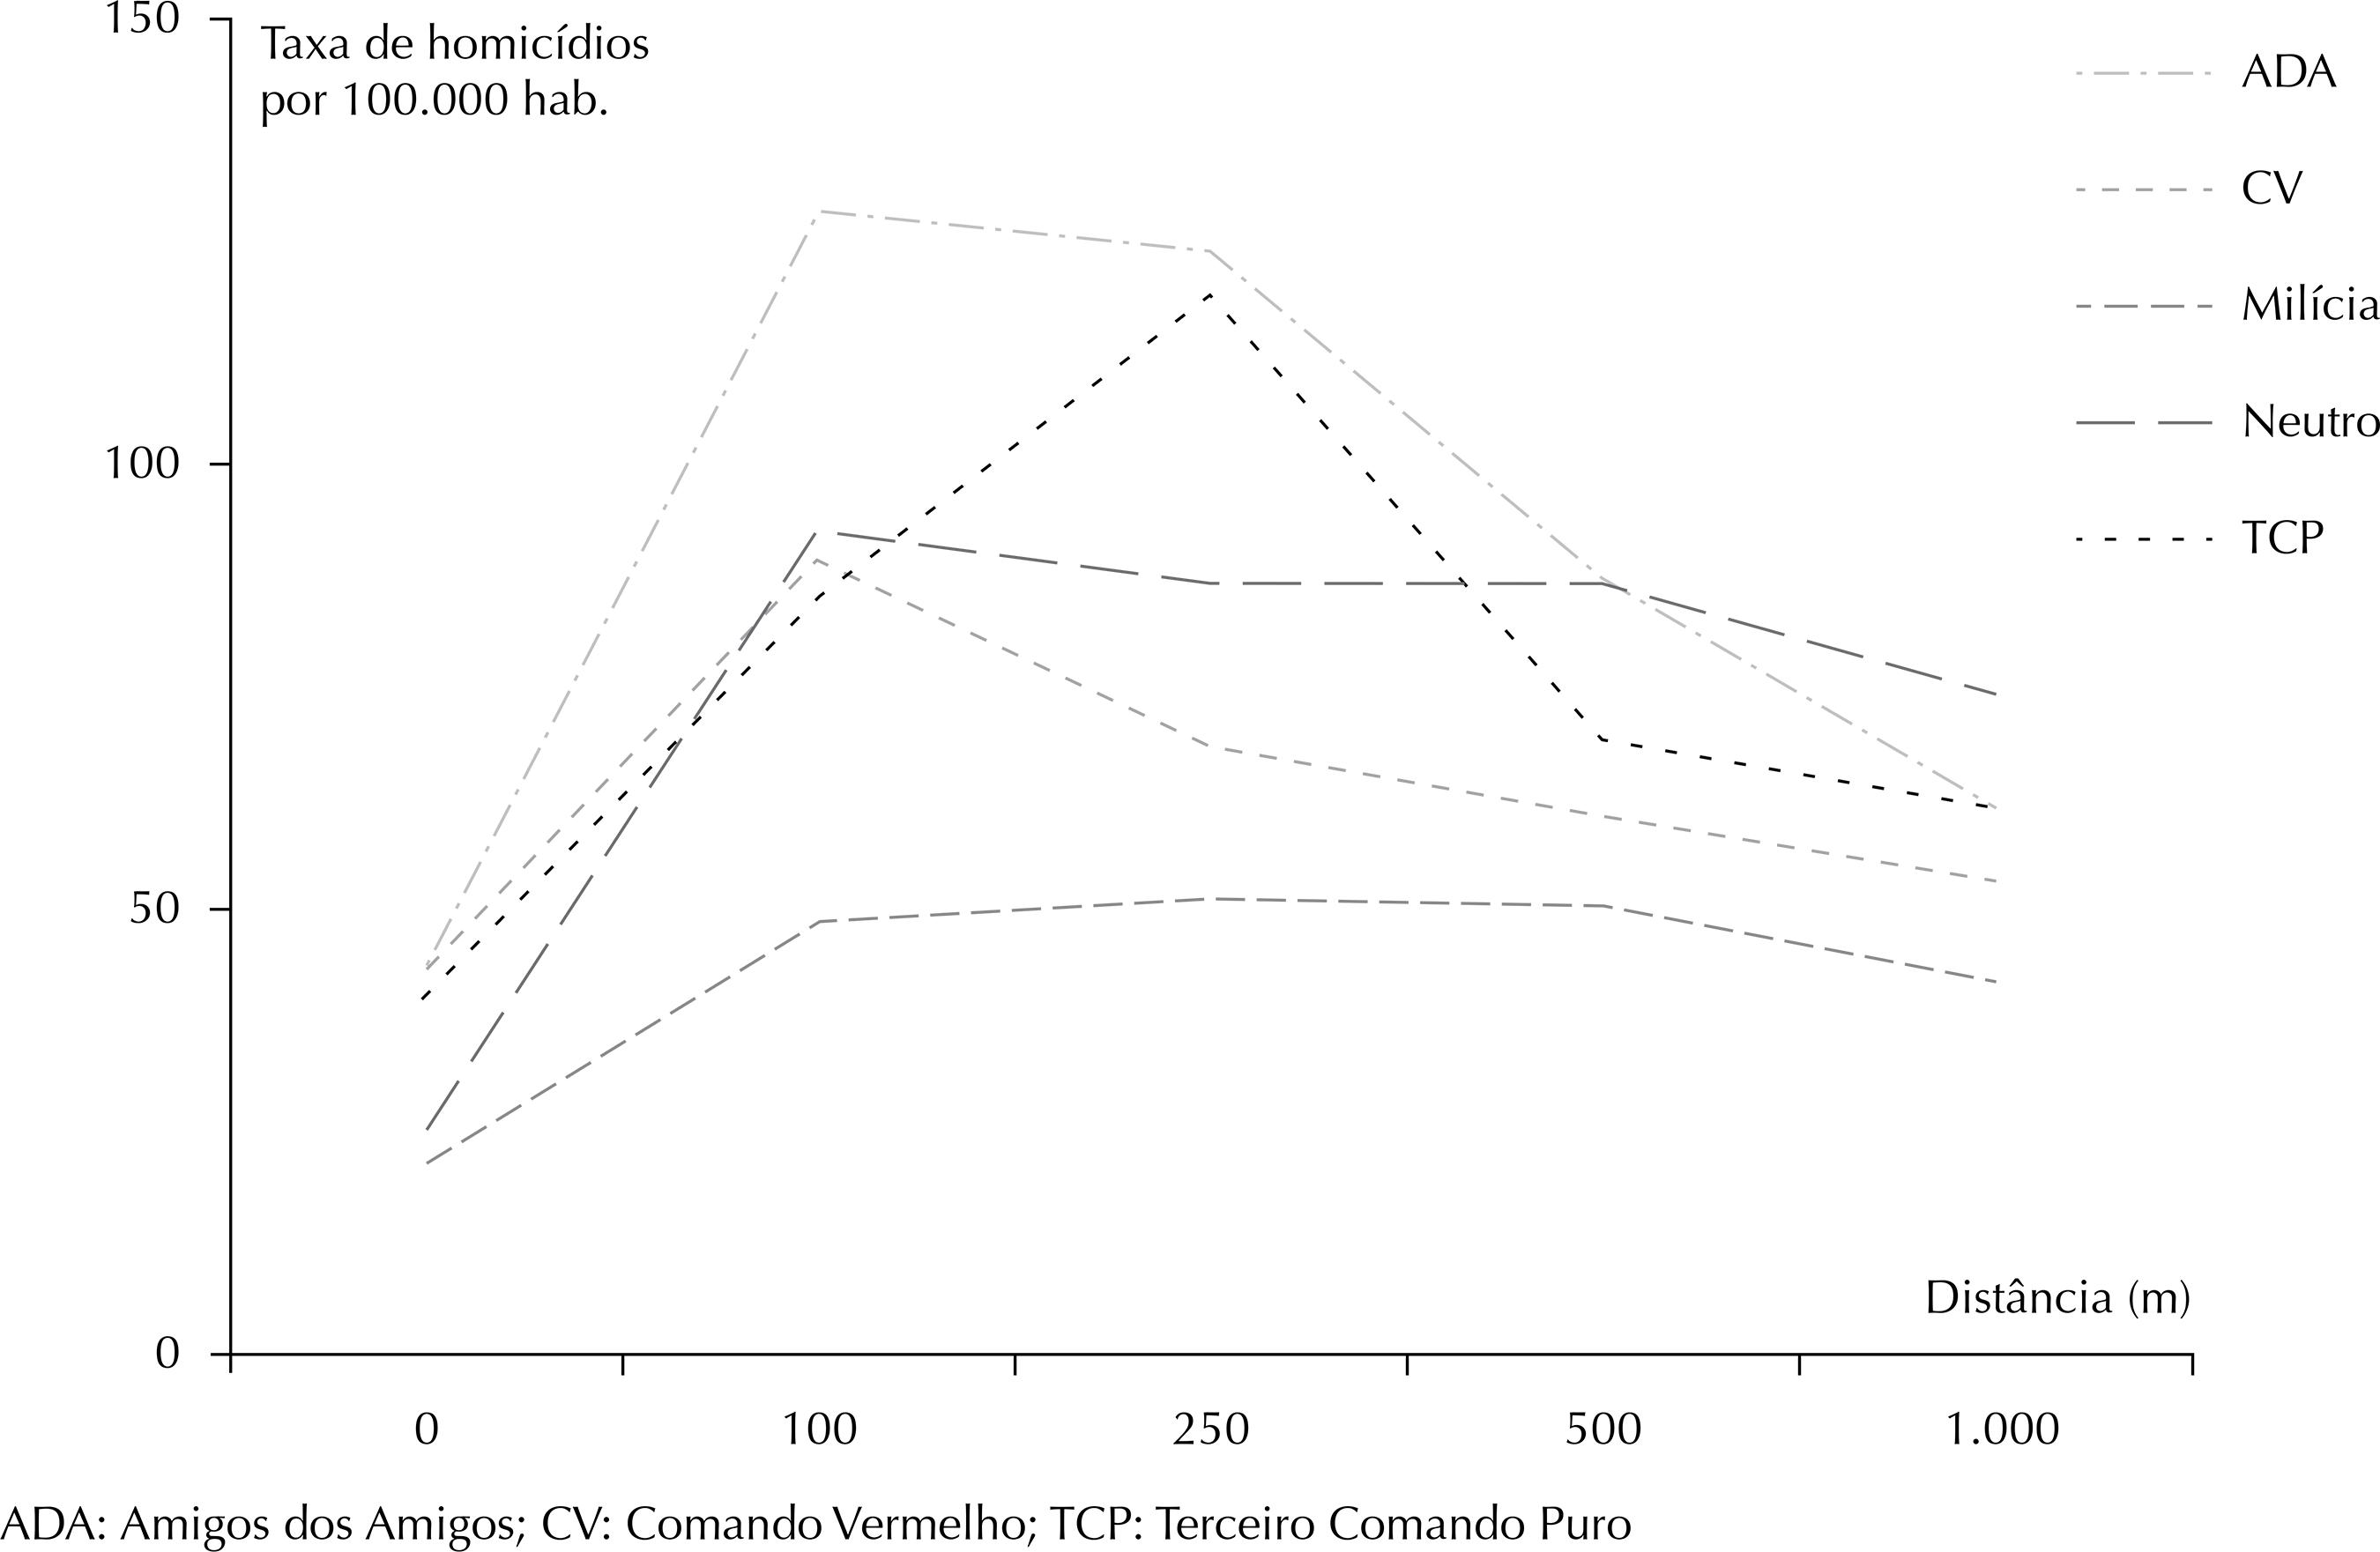
\includegraphics[width=\textwidth]{0034-8910-rsp-48-01-0094-gf02}
\caption{}\label{fig:f02}
\end{figure}
\begin{figure}
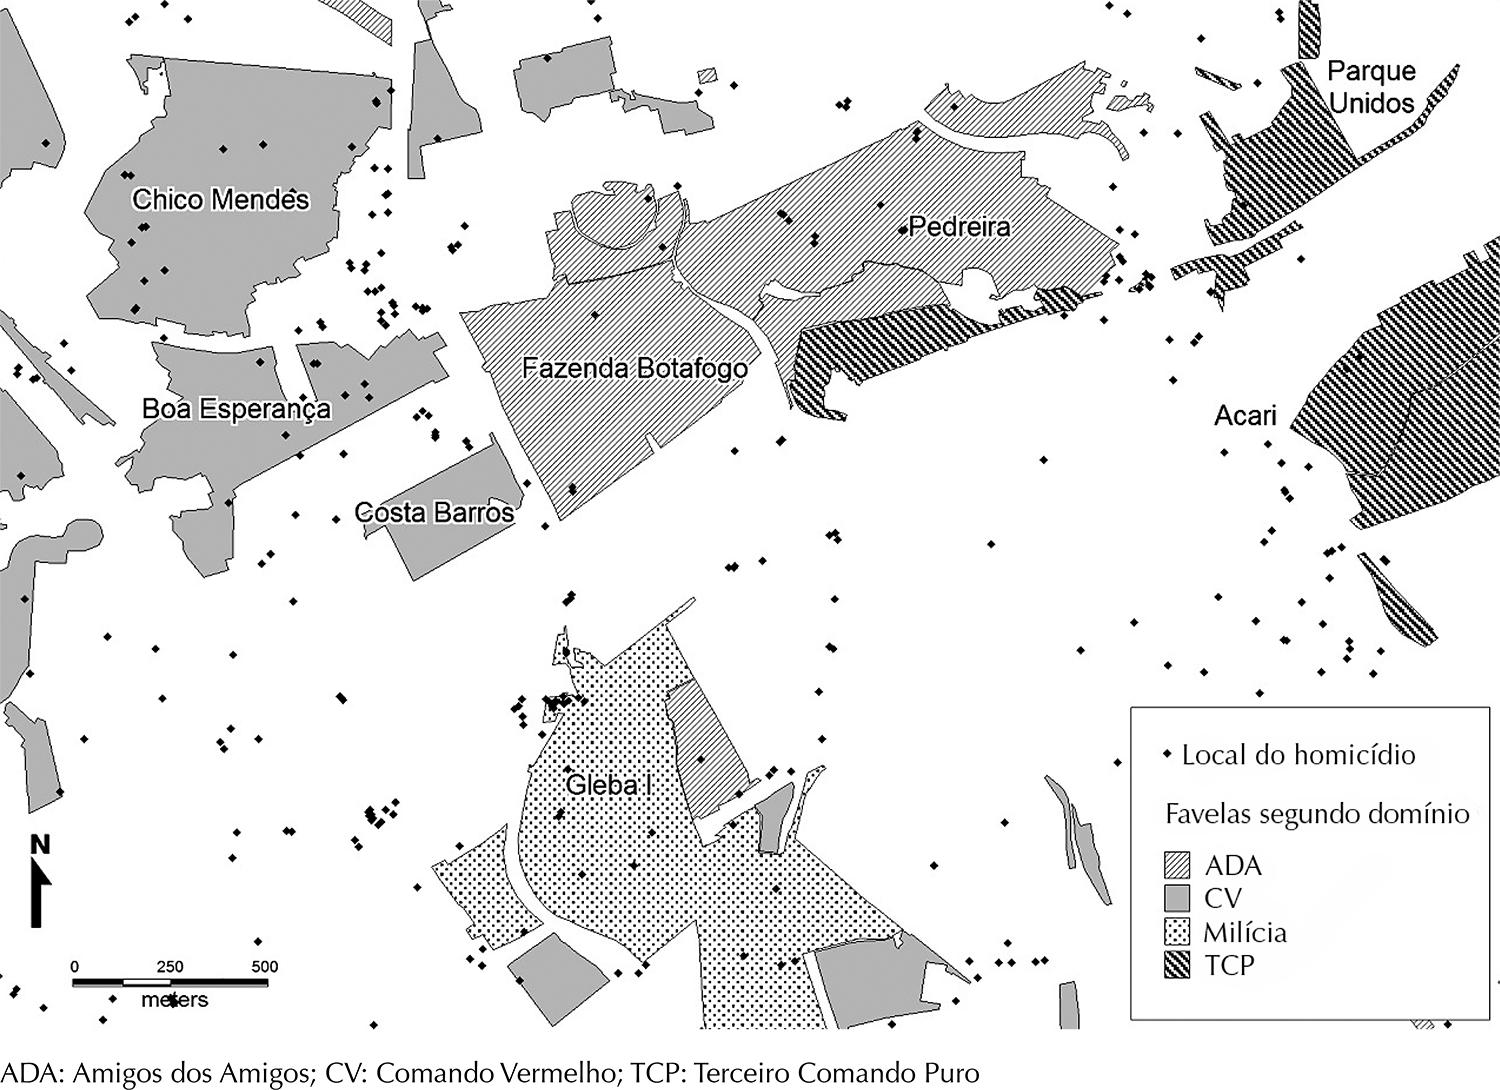
\includegraphics[width=\textwidth]{0034-8910-rsp-48-01-0094-gf03}
\caption{}\label{fig:f03}
\end{figure}

\section{\textsc{discussão}}

Estas análises demonstram que morar em favelas não representa, por si, um
sobre-risco de morte por homicídio. Este risco é determinado pela dinâmica de
ocupação destes territórios e a presença de armas e grupos criminosos,
especialmente os vinculados ao tráfico ilegal de drogas. As disputas
territoriais estão alterando a configuração espacial do tráfico de drogas no Rio
de Janeiro, que têm consequências importantes sobre o homicídio. As zonas de
conflito, onde favelas estão próximas a centros de abastecimento, portos e
aeroportos, ou onde há uma proximidade entre facções criminosas rivais,
apresentam maiores taxas de homicídio.

As principais mudanças de domínios ocorreram nas zonas sul e norte da cidade,
pela ocupação das \textsc{upp} nestas áreas, e na zona oeste, devido à tomada de favelas
pelas milícias.\textsuperscript{[}\textsuperscript{22}\textsuperscript{]}
Até 2005, as milícias estavam restritas à zona oeste, áreas de povoamento mais
recente, de menor densidade populacional e com percentual alto de migrantes
nordestinos entre os moradores. Em 2010, as milícias haviam se expandido para
outras áreas dos chamados subúrbios, mas não nas favelas próximas a uma das
principais avenidas da cidade. As únicas favelas que permaneceram sob o domínio
do CV na zona oeste, em 2009, estavam localizadas em Cidade de Deus. Na zona sul
da cidade, mais próspera com famílias de renda alta, nenhuma favela foi dominada
pela milícia. A restrição das áreas de atuação das milícias pode ser
consequência da morfologia da cidade, devido às dificuldades de circulação por
conta das montanhas e do mar, ao contrário da zona oeste, mais plana, que
facilitaria a movimentação dos paramilitares. Uma segunda hipótese, baseada em
pesquisas anteriores,\textsuperscript{[}\textsuperscript{25}\textsuperscript{]}
é a de que muitas das empresas de segurança, uniformizadas ou não, nas áreas
mais prósperas da cidade pertencem a policiais, que também atuam como “milícias”
nas áreas pobres. A grande diferença estaria na relação do pessoal da segurança
com os moradores. Nas áreas pobres, pela falta de acesso à justiça, mais
facilmente os agentes da segurança privada tornam-se tiranos ou negociantes que
impõem decisões extralegais ou ilegais aos moradores pelo poder advindo das
armas, afastando assaltantes e traficantes do local.

A presença do tráfico, principalmente o tráfico armado, aumenta as taxas de
homicídios no entorno de favelas. Grande parte deles decorre de conflitos
armados entre traficantes de diferentes comandos, entre estes e as polícias, ou
entre traficantes e milicianos pela conquista ou defesa de territórios ou pela
cobrança de dívidas e de propinas. O porte de armas de fogo, por sua vez, se
explica pelo contexto sociocultural dos pequenos grupos aos quais pertencem os
jovens que seguem os valores e práticas desta cultura de rua. Alguns estudos,
sobretudo nos Estados Unidos, apontam o grupo de pares como o maior preditivo de
delinquência entre homens jovens, especialmente os crimes violentos mais graves
e o hábito de portar armas.\textsuperscript{[}\textsuperscript{14}\textsuperscript{]}
Outros estudos afirmam que carregar arma e repetência na escola são os
preditores de violência mais importantes para
jovens.\textsuperscript{[}\textsuperscript{8}\textsuperscript{]}\textsuperscript{,}\textsuperscript{[}\textsuperscript{15}\textsuperscript{]}
O aumento da taxa de homicídios é melhor explicado pela alta concentração de
armas onde homens jovens e pobres vivem, do que pela inclinação natural à
violência.

Os altos valores de taxas de homicídio encontrados nas imediações de favelas
podem ter duas explicações não excludentes. Há grande dificuldade de se
localizar endereços de residência no interior de
favelas.\textsuperscript{[}\textsuperscript{1}\textsuperscript{]}
O padrão de arruamento e a informalidade dos logradouros muitas vezes impede que
se localizem endereços em becos e vielas nas favelas. Uma estratégia adotada
pelos moradores é fornecer endereços nas vizinhanças, como sedes de associação
de moradores, lojas e outros locais de referência em áreas formais. Isso faz com
que os endereços declarados nos sistemas de informação, tanto da segurança
pública quanto da saúde, sejam localizados nos arredores das favelas, aumentado
artificialmente os riscos estimados para essas áreas.

Uma segunda explicação é a ampliação dos conflitos nas fronteiras das favelas. O
aumento das taxas em áreas vizinhas pode ocorrer pela existência de conflitos
territoriais entre grupos criminosos e a proibição, pelos traficantes, da
prática de assaltos dentro da favela, embora aceitem armas e dinheiro dos
ladrões. Essas práticas são muito comuns em cidades brasileiras onde o tráfico
de drogas armado ocupa e defende seus
territórios.\textsuperscript{[}\textsuperscript{4}\textsuperscript{]}\textsuperscript{,}\textsuperscript{[}\textsuperscript{7}\textsuperscript{]}\textsuperscript{,}\textsuperscript{[}\textsuperscript{24}\textsuperscript{]}

O domínio de favelas por \textsc{upp} ou milícias aparentemente reduz os riscos de
mortalidade por violência. Em anos mais recentes houve um considerável
crescimento deste tipo de ocupação de favelas na cidade. As estimativas
preliminares permitem verificar uma tendência de proteção dos seus moradores
quando a favela está submetida a uma \textsc{upp}.

As áreas dominadas por milícias apresentam menores taxas de mortalidade por
violência que áreas sob domínio de grupos armados de tráfico. A estratégia de
ocupação destas áreas poderia explicar esta diferença. As milícias não ocupam
somente as favelas, mas todo seu entorno, que se torna fonte lucrativa de renda
obtida por comércio legal ou ilegal de bens e serviços como transporte, energia,
água, lazer, entre outros. Além disso, as milícias empregam outras formas de
coerção aos moradores, como banir pessoas ligadas ao tráfico, recolher armas,
torturar pessoas que cometeram crimes considerados inaceitáveis, entre outras
práticas.

As técnicas de análise espacial permitiram avaliar as condições de risco de
populações vulneráveis, não considerando as favelas como fenômeno sócio-espacial
homogêneo, mas segundo diferentes formas de ocupação e atuação de grupos
armados. A análise permitiu confirmar a hipótese de que os domínios de tráfico e
a presença de grupos armados aumentam os riscos de mortes por agressão.

Esta hipótese foi corroborada por depoimentos colhidos com os moradores de
favelas que relataram práticas de violência existentes em favelas dominadas por
tais grupos, práticas que não afetam somente criminosos, mas moradores, na
favela e arredores, que podem ser vítimas de homicídios devido à prevalência do
\textit{ethos}
da masculinidade violenta, a disponibilidade de armas, e a coerção e o domínio
sobre estes territórios, caracterizando a “ecologia do perigo” no entorno de
favelas dominadas pelo tráfico e localizadas em zonas estratégicas da cidade.

TabelaPopulação estimada, número de homicídios segundo local de residência da
vítima e taxa de homicídio segundo o tipo de atividade no entorno próximo de
favelas do Rio de Janeiro, RJ, 2009.\begin{table}
\begin{adjustbox}{width=1.1\textwidth}
\small
\begin{tabulary}{\linewidth}{ C C C C C C C }
\hline
Tipo de ocupação & População estimada &\textsuperscript{a}
& Número de homicídios &\textsuperscript{b}
& Taxa homicídios (por 100.000 hab.) &\textsuperscript{c}
\\ \hline
Com domínio armada
& 3.130.117
& 1.585
& 50,6
\\ \hline

Com domínio desarmada
& 287.315
& 131
& 45,6
\\ \hline

Com domínio com tráfico
& 167.764
& 120
& 71,5
\\ \hline

Sem domínio sem tráfico
& 17.862
& 4
& 22,4
\\ \hline

\end{tabulary}
\end{adjustbox}
\caption{}
\end{table}\textsuperscript{a}
\textsc{ibge}. Censo demográfico, 2010.\textsuperscript{b}
Secretaria Municipal de Saúde do Rio de Janeiro, 2006 a 2009.\textsuperscript{c}
Distância de até 250 m.\textsuperscript{a}
\textsc{ibge}. Censo demográfico, 2010.\textsuperscript{b}
Secretaria Municipal de Saúde do Rio de Janeiro, 2006 a 2009.\textsuperscript{c}
Distância de até 250 m.

\section*{\textsc{referências}}
\begin{itemize}

\item[1] Barcellos C, Ramalho WM, Gracie R, Magalhães \textsc{mafm}, Fontes MP, Skaba D.
Georreferenciamento de dados de saúde na escala submunicipal: algumas
experiências no Brasil. \textit{Epidemiol Serv Saude}. 2008;17(1):59-70.

\item[2] Beato Filho CC, Assunção RM, Silva \textsc{bfa}, Marinho FC, Reis IA, Almeida
MC. Conglomerados de homicídios e o tráfico de drogas em Belo Horizonte, Minas
Gerais, Brasil, de 1995 a 1999. \textit{Cad Saude Publica}. 2001;17(5):1163-71. \textsc{doi}:10.1590/S0102-311X2001000500017

\item[3] Burawoy M. The extended case method. \textit{Sociol Theory}. 1998;16(1):4-33. \textsc{doi}:10.1111/0735-2751.00040

\item[4] Cano I, Santos N. Violência letal, renda e desigualdade social no
Brasil. Rio de Janeiro: 7 Letras; 2001.

\item[5] Castro \textsc{msm}, Assunção RM, Durante MO. Comparação de dados sobre
homicídios entre dois sistemas de informação, Minas Gerais. \textit{Rev Saude
Publica}. 2003;37(2):168-76. \textsc{doi}:10.1590/S0034-89102003000200002

\item[6] Chainey S, Ratcliffe J. \textsc{gis} and crime mapping. London: John Wiley \&
Sons; 2005.

\item[7] Dowdney L. Crianças no tráfico: um estudo de caso de crianças em
violência armada organizada no Rio de Janeiro. Rio de Janeiro: 7 Letras; 2003.

\item[8] Ellikson P, Saner H, McGuigan KA. Profiles of violent youth: substance
use and other concurrent problems. \textit{Am J Public Health}. 1997;87(6):985-91.

\item[9] Fagan J. Policing guns and youth violence. \textit{Future Child}. 2005;12(2):133-51.

\item[10] Gawryszewski VP, Costa LS. Social inequality and homicide rates in Sao
Paulo City, Brazil. \textit{Rev Saude Publica}. 2005;39(2):191-7. \textsc{doi}:10.1590/S0034-89102005000200008

\item[11] Iyer S, Monteiro \textsc{mfg}. The risk of child and adolescent mortality among
vulnerable populations. \textit{J Biosoc Sci}. 2004;36(5):523-46.

\item[12] Melgaço LM. Uso do território pela violência. In: Souza MA,
organizadora. Território brasileiro: usos e abusos. Campinas: Edições
Territorial; 2003. v.1, p.524-33.

\item[13] Misse M. La acumulación social de la violencia en Rio de Janeiro y en
Brasil: algunas reflexiones. \textit{Co- Herencia}. 2010;7(13):19-40.

\item[14] Myers GP, McGrady GA, Marrow C, Mueller CW. Weapon carrying among
black adolescents: a social network perspective. \textit{Am J Public Health}. 1997;87(6):1038-40.

\item[15] Resnick MD, Ireland M, Borowsky I. Youth violence perpetration: what
protects? What predicts? Findings from the National Longitudinal Study of
Adolescent Health. \textit{J Adolesc Health}. 2004;35(5):424.e1-424.e10. \textsc{doi}:10.1016/j.jadohealth.2004.01.011

\item[16] Rojas LI; Santos SM; Barcellos C. Diferenciación espacial de la
violencia en America Latina. In: Minayo \textsc{mcs}, Coimbra Jr \textsc{cea}, organizadores.
Críticas e atuantes: ciências sociais e humanas em saúde na América Latina. Rio
de Janeiro: Editora. Fiocruz; 2005. p.665-86.

\item[17] Santos M. A natureza do espaço: técnica e tempo, razão e emoção. São
Paulo: Hucitec; 1996.

\item[18] Santos SM, Barcellos C, Sá Carvalho M. Ecological analysis of the
distribution and socio-spatial context of homicides in Porto Alegre, Brazil.
\textit{Health Place}. 2006;12(1):38-47. \textsc{doi}:10.1016/j.healthplace.2004.08.009

\item[19] Soares Filho AM. Homicide victimization according to racial
characteristics in Brazil. \textit{Rev Saude Publica}. 2011;45(4):745-55. \textsc{doi}:10.1590/S0034-89102011005000045

\item[20] Szwarcwald CL, Bastos FI, Esteves MA, Andrade \textsc{clt}, Paez MS, Medici EV,
et al. Desigualdades de renda e situação de saúde: o caso do Rio de Janeiro.
\textit{Cad Saude Publica}. 1999;15(1):15-28.\textsc{doi}:10.1590/S0102-311X1999000100003

\item[21] Taquette S, Caldas CP, organizadoras. Ética e pesquisa com populações
vulneráveis. Rio de Janeiro: Editora da Universidade do Estado do Rio de
Janeiro; 2012. pág. 46

\item[22] Zaluar A, Barcellos C. Mortes prematuras e conflito armado pelo
domínio das favelas no Rio de Janeiro. \textit{Rev Bras Cienc Soc}. 2013;28(81):17-31. \textsc{doi}:10.1590/S0102-69092013000100002

\item[23] Zaluar A. Turf war in Rio de Janeiro: youth, drug traffic, guns and
hyper-masculinity. In:Ceccato V, editor. The urban fabric of crime and fear. New
York: Springer; 2012. v.1, p.217-38.

\item[24] Zaluar A. Violence in Rio de Janeiro: styles of leisure, drug use, and
trafficking. \textit{Int Soc Sci J}. 2001;53(3):369-78.

\item[25] Zaluar AM, Conceição IS. Favelas sob o controle das milícias no Rio de
Janeiro: que paz? \textit{Sao Paulo Perspect}. 2007;21(2):89-101.

\item[26] Zaluar AM. Pesquisando no perigo: etnografias voluntárias e não
acidentais. \textit{Mana}. 2009;15(2):557-84. \textsc{doi}:10.1590/S0104-93132009000200009

\end{itemize}

   \section*{Metadados não aplicados}
    \begin{itemize}
    \ifdef{\lingua}{\item[\textbf{língua do artigo}] \lingua}{}
    \ifdef{\journalid}{\item[\textbf{journalid}] \journalid}{}
    \ifdef{\journaltitle}{\item[\textbf{journaltitle}] \journaltitle}{}
    \ifdef{\journalsubtitle}{\item[\textbf{journalsubtitle}] \journalsubtitle}{}
    \ifdef{\historydateaccepted}{\item[\textbf{historydateaccepted}] \historydateaccepted}{}
    \ifdef{\historydatereceived}{\item[\textbf{historydatereceived}] \historydatereceived}{}
    \ifdef{\ack}{\item[\textbf{ack}] \ack}{}
    \ifdef{\transjournaltitle}{\item[\textbf{journaltitle}] \journaltitle}{}
    \ifdef{\transjournalsubtitle}{\item[\textbf{journalsubtitle}] \journaltitle}{}
    \ifdef{\abbrevjournaltitle}{\item[\textbf{abbrevjournaltitle}] \abbrevjournaltitle}{}
    \ifdef{\issnppub}{\item[\textbf{issnppub}] \issnppub}{}
    \ifdef{\issnepub}{\item[\textbf{issnepub}] \issnepub}{}
    \ifdef{\alttitleauthor}{\item[\textbf{alttitle}] \alttitleauthor}{}
    \ifdef{\alttitle}{\item[\textbf{alttitleauthor}] \alttitle}{}
    \ifdef{\publishername}{\item[\textbf{publishername}] \publishername}{}
    \ifdef{\publisherid}{\item[\textbf{publisherid}] \publisherid}{}
    \ifdef{\subject}{\item[\textbf{subject}] \subject}{} 
    \ifdef{\transtitle}{\item[\textbf{transtitle}] \transtitle}{}
    \ifdef{\authornotes}{\item[\textbf{authornotes}] \authornotes}{}
    \ifdef{\articleid}{\item[\textbf{articleid}] \articleid}{}
    \ifdef{\articledoi}{\item[\textbf{articledoi}] \articledoi}{}
    \ifdef{\volume}{\item[\textbf{volume}] \volume}{}
    \ifdef{\issue}{\item[\textbf{issue}] \issue}{}
    \ifdef{\fpage}{\item[\textbf{fpage}] \fpage}{}
    \ifdef{\lpage}{\item[\textbf{lpage}] \lpage}{}
    \ifdef{\permissions}{\item[\textbf{permissions}] \permissions}{}
    \ifdef{\copyrightyear}{\item[\textbf{copyrightyear}] \copyrightyear}{}

    \end{itemize}
\end{document}
